\documentclass[spanish,]{book}
\usepackage{lmodern}
\usepackage{amssymb,amsmath}
\usepackage{ifxetex,ifluatex}
\usepackage{fixltx2e} % provides \textsubscript
\ifnum 0\ifxetex 1\fi\ifluatex 1\fi=0 % if pdftex
  \usepackage[T1]{fontenc}
  \usepackage[utf8]{inputenc}
\else % if luatex or xelatex
  \ifxetex
    \usepackage{mathspec}
  \else
    \usepackage{fontspec}
  \fi
  \defaultfontfeatures{Ligatures=TeX,Scale=MatchLowercase}
\fi
% use upquote if available, for straight quotes in verbatim environments
\IfFileExists{upquote.sty}{\usepackage{upquote}}{}
% use microtype if available
\IfFileExists{microtype.sty}{%
\usepackage{microtype}
\UseMicrotypeSet[protrusion]{basicmath} % disable protrusion for tt fonts
}{}
\usepackage{hyperref}
\hypersetup{unicode=true,
            pdftitle={Introducción al Análisis de Datos},
            pdfauthor={Matías Alfonso},
            pdfborder={0 0 0},
            breaklinks=true}
\urlstyle{same}  % don't use monospace font for urls
\ifnum 0\ifxetex 1\fi\ifluatex 1\fi=0 % if pdftex
  \usepackage[shorthands=off,main=spanish]{babel}
\else
  \usepackage{polyglossia}
  \setmainlanguage[]{spanish}
\fi
\usepackage{natbib}
\bibliographystyle{apalike}
\usepackage{color}
\usepackage{fancyvrb}
\newcommand{\VerbBar}{|}
\newcommand{\VERB}{\Verb[commandchars=\\\{\}]}
\DefineVerbatimEnvironment{Highlighting}{Verbatim}{commandchars=\\\{\}}
% Add ',fontsize=\small' for more characters per line
\usepackage{framed}
\definecolor{shadecolor}{RGB}{248,248,248}
\newenvironment{Shaded}{\begin{snugshade}}{\end{snugshade}}
\newcommand{\KeywordTok}[1]{\textcolor[rgb]{0.13,0.29,0.53}{\textbf{#1}}}
\newcommand{\DataTypeTok}[1]{\textcolor[rgb]{0.13,0.29,0.53}{#1}}
\newcommand{\DecValTok}[1]{\textcolor[rgb]{0.00,0.00,0.81}{#1}}
\newcommand{\BaseNTok}[1]{\textcolor[rgb]{0.00,0.00,0.81}{#1}}
\newcommand{\FloatTok}[1]{\textcolor[rgb]{0.00,0.00,0.81}{#1}}
\newcommand{\ConstantTok}[1]{\textcolor[rgb]{0.00,0.00,0.00}{#1}}
\newcommand{\CharTok}[1]{\textcolor[rgb]{0.31,0.60,0.02}{#1}}
\newcommand{\SpecialCharTok}[1]{\textcolor[rgb]{0.00,0.00,0.00}{#1}}
\newcommand{\StringTok}[1]{\textcolor[rgb]{0.31,0.60,0.02}{#1}}
\newcommand{\VerbatimStringTok}[1]{\textcolor[rgb]{0.31,0.60,0.02}{#1}}
\newcommand{\SpecialStringTok}[1]{\textcolor[rgb]{0.31,0.60,0.02}{#1}}
\newcommand{\ImportTok}[1]{#1}
\newcommand{\CommentTok}[1]{\textcolor[rgb]{0.56,0.35,0.01}{\textit{#1}}}
\newcommand{\DocumentationTok}[1]{\textcolor[rgb]{0.56,0.35,0.01}{\textbf{\textit{#1}}}}
\newcommand{\AnnotationTok}[1]{\textcolor[rgb]{0.56,0.35,0.01}{\textbf{\textit{#1}}}}
\newcommand{\CommentVarTok}[1]{\textcolor[rgb]{0.56,0.35,0.01}{\textbf{\textit{#1}}}}
\newcommand{\OtherTok}[1]{\textcolor[rgb]{0.56,0.35,0.01}{#1}}
\newcommand{\FunctionTok}[1]{\textcolor[rgb]{0.00,0.00,0.00}{#1}}
\newcommand{\VariableTok}[1]{\textcolor[rgb]{0.00,0.00,0.00}{#1}}
\newcommand{\ControlFlowTok}[1]{\textcolor[rgb]{0.13,0.29,0.53}{\textbf{#1}}}
\newcommand{\OperatorTok}[1]{\textcolor[rgb]{0.81,0.36,0.00}{\textbf{#1}}}
\newcommand{\BuiltInTok}[1]{#1}
\newcommand{\ExtensionTok}[1]{#1}
\newcommand{\PreprocessorTok}[1]{\textcolor[rgb]{0.56,0.35,0.01}{\textit{#1}}}
\newcommand{\AttributeTok}[1]{\textcolor[rgb]{0.77,0.63,0.00}{#1}}
\newcommand{\RegionMarkerTok}[1]{#1}
\newcommand{\InformationTok}[1]{\textcolor[rgb]{0.56,0.35,0.01}{\textbf{\textit{#1}}}}
\newcommand{\WarningTok}[1]{\textcolor[rgb]{0.56,0.35,0.01}{\textbf{\textit{#1}}}}
\newcommand{\AlertTok}[1]{\textcolor[rgb]{0.94,0.16,0.16}{#1}}
\newcommand{\ErrorTok}[1]{\textcolor[rgb]{0.64,0.00,0.00}{\textbf{#1}}}
\newcommand{\NormalTok}[1]{#1}
\usepackage{longtable,booktabs}
\usepackage{graphicx,grffile}
\makeatletter
\def\maxwidth{\ifdim\Gin@nat@width>\linewidth\linewidth\else\Gin@nat@width\fi}
\def\maxheight{\ifdim\Gin@nat@height>\textheight\textheight\else\Gin@nat@height\fi}
\makeatother
% Scale images if necessary, so that they will not overflow the page
% margins by default, and it is still possible to overwrite the defaults
% using explicit options in \includegraphics[width, height, ...]{}
\setkeys{Gin}{width=\maxwidth,height=\maxheight,keepaspectratio}
\IfFileExists{parskip.sty}{%
\usepackage{parskip}
}{% else
\setlength{\parindent}{0pt}
\setlength{\parskip}{6pt plus 2pt minus 1pt}
}
\setlength{\emergencystretch}{3em}  % prevent overfull lines
\providecommand{\tightlist}{%
  \setlength{\itemsep}{0pt}\setlength{\parskip}{0pt}}
\setcounter{secnumdepth}{5}
% Redefines (sub)paragraphs to behave more like sections
\ifx\paragraph\undefined\else
\let\oldparagraph\paragraph
\renewcommand{\paragraph}[1]{\oldparagraph{#1}\mbox{}}
\fi
\ifx\subparagraph\undefined\else
\let\oldsubparagraph\subparagraph
\renewcommand{\subparagraph}[1]{\oldsubparagraph{#1}\mbox{}}
\fi

%%% Use protect on footnotes to avoid problems with footnotes in titles
\let\rmarkdownfootnote\footnote%
\def\footnote{\protect\rmarkdownfootnote}

%%% Change title format to be more compact
\usepackage{titling}

% Create subtitle command for use in maketitle
\providecommand{\subtitle}[1]{
  \posttitle{
    \begin{center}\large#1\end{center}
    }
}

\setlength{\droptitle}{-2em}

  \title{Introducción al Análisis de Datos}
    \pretitle{\vspace{\droptitle}\centering\huge}
  \posttitle{\par}
    \author{Matías Alfonso}
    \preauthor{\centering\large\emph}
  \postauthor{\par}
      \predate{\centering\large\emph}
  \postdate{\par}
    \date{2019-09-10}

\usepackage{booktabs}
\usepackage{amsthm}
\makeatletter
\def\thm@space@setup{%
  \thm@preskip=8pt plus 2pt minus 4pt
  \thm@postskip=\thm@preskip
}
\makeatother

\begin{document}
\maketitle

{
\setcounter{tocdepth}{1}
\tableofcontents
}
\part{Programación en R}\label{part-programacion-en-r}

\chapter{Preliminares}\label{prelim}

R es un lenguaje de programación desarrollado inicialmente por Ross
Ihaka y Robert Gentleman en el departamento de Estadística de la
Universidad de Auckland en 1993. Está orientado específicamente con un
enfoque al análisis estadístico.\\
R se desarrolla a partir de un lenguaje denominado S, desarrollado por
John Chambers en 1976, disponible a partir del software comercial
S-PLUS.\\
Es un lenguaje interactivo, permite la ejecución de instrucciónes en
líneas de comando en una consola.

\section{¿Por qué R?}\label{por-que-r}

R puede ser ejecutado en múltiples plataformas y en la gran mayoría de
los sistemas operativos. Puede ser ejecutado en tablets, teléfonos o
computadoras. La utilización de scripts permite compartir fácilmente los
análisis con los colegas, así como asegurar la reproductibilidad de los
resultados. Todo lo que realizamos mediante una interfaz gráfica con el
mouse no deja registros de nuestro trabajo e impide que podamos repasar
nuestro trabajo para corregir errores.\\
La versatilidad y la potencia que otorga un lenguaje de programación es
mucho mayor que la que podemos obtener con softwares estadísticos de
interfaz gráfica.\\
La comunidad de usuarios y desarrolladores de R está en constante
crecimiento en los últimos años. Hay una enorme cantidad de gente
realizando nuevos desarrollos en R cada día, que están a la vanguardia
de la ciencia computacional y estadística.

\section{Software Libre}\label{software-libre}

La mayor ventaja que tiene R con respecto a otros softwares de análisis
estadístico es que es un software libre. ¿Qué quiere decir eso? Por un
lado, que es gratuito. Por otro, que el código fuente con el que R fue
desarrollado está abierto, se puede descargar y está diponible online.
Actualmente el copyrigth de R lo posee la
\href{https://www.r-project.org/foundation/}{R Foundation}. R forma
parte del \href{https://es.wikipedia.org/wiki/GNU}{sistema GNU},
desarrollado por la
\href{https://es.wikipedia.org/wiki/Free_Software_Foundation}{Free
Software Foundation}. De acuerdo a la Free Software Foundation, con el
software libre se garantizan cuatro libertades fundamentales:

\begin{itemize}
\tightlist
\item
  La libertad de ejecutar el programa para cualquier propósito.
  (Libertad 0)
\item
  La libertad de estudiar cómo el programa funciona y adaptarlo a tus
  propias necesidades. (Libertad 1)
\item
  La libertad de redistribuir copias de manera que puedas ayudar a
  alguien. (Libertad 2)
\item
  La libertad de mejorar el programa, y liberar tus mejoras al público,
  de manera que se beneficie toda la comunidad. (Libertad 3)
\end{itemize}

\section{Sistema de Paquetes}\label{sistema-de-paquetes}

El sistema de funcionalidades de R se encuentra agrupado en paquetes. La
mayor parte de los paquetes se encuentran disponibles en
\href{https://cran.r-project.org/}{Comprehensive R Archive Network
(CRAN)}. Hay un conjunto de paquetes principales, de base, que incluye
todos los paquetes que se instalan por defecto cuando instalamos R.
Luego, tenemos un montón de paquetes con funcionalidades específicas que
podemos instalar en función de nuestras necesidades.

\chapter{Primeros pasos}\label{primeros-pasos}

\section{Asignación de datos y
evaluación.}\label{asignacion-de-datos-y-evaluacion.}

R es un \emph{lenguaje interpretado}. Esto quiere decir que le podemos
ir pasando instrucciones y el programama las irá interpretando. Cuando
ejecutamos el programa, nos encontramos con el prompt a la espera de
intrucciones:

\begin{verbatim}
>
\end{verbatim}

Una de las operaciones más sencillas que podemos realizar es la
asignación de valores a las variables. El operador de asignación es
\texttt{\textless{}-}.

\begin{Shaded}
\begin{Highlighting}[]
\NormalTok{x <-}\StringTok{ }\DecValTok{1}
\KeywordTok{print}\NormalTok{(x)}
\end{Highlighting}
\end{Shaded}

\begin{verbatim}
## [1] 1
\end{verbatim}

\begin{Shaded}
\begin{Highlighting}[]
\NormalTok{x}
\end{Highlighting}
\end{Shaded}

\begin{verbatim}
## [1] 1
\end{verbatim}

\begin{Shaded}
\begin{Highlighting}[]
\NormalTok{texto <-}\StringTok{ "hola mundo"}
\NormalTok{texto}
\end{Highlighting}
\end{Shaded}

\begin{verbatim}
## [1] "hola mundo"
\end{verbatim}

Podemos imprimir el valor de una variable con la función
\texttt{print()} o directamente escribiendo la variable.

Tenemos dos formas de interactuar con R:

\begin{itemize}
\tightlist
\item
  Tipear directamente los comandos en el prompt y ejecutarlos.
\item
  Escribir un archivo de texto con todas las intrucciones y luego
  ejecutarlo. Este archivo se denomina script.
\end{itemize}

\section{Working directory}\label{working-directory}

Lo primero que debemos hacer cuando comenzamos a trabajar en R es
configurar el directorio de trabajo. Una buena costumbre es crear un
directorio nuevo de trabajo cuando comenzamos un proyecto nuevo. Luego
configuramos esa carpeta como directorio de trabajo. Colocamos allí
todos los archivos vinculados a ese proyecto. Para determinar en qué
directorio estamos parados, podemos utilizar el comando
\texttt{getwd()}. Para configurar el directorio de trabajo, utilizamos

\begin{verbatim}
setwd(#RUTA-A-DIRECTORIO)
\end{verbatim}

\section{Comentarios}\label{comentarios}

Todo lo que escribamos luego de un \texttt{\#} en una intrucción, no
será evaluado.

\begin{Shaded}
\begin{Highlighting}[]
\NormalTok{x <-}\StringTok{ }\KeywordTok{c}\NormalTok{(}\DecValTok{3}\NormalTok{, }\DecValTok{4}\NormalTok{, }\DecValTok{5}\NormalTok{)}
\NormalTok{## Esto no se ejecuta}

\NormalTok{x}
\end{Highlighting}
\end{Shaded}

\begin{verbatim}
## [1] 3 4 5
\end{verbatim}

Ello nos permite comentar el código que escribimos, a manera de
documentación.

\section{Objetos básicos en R}\label{objetos-basicos-en-r}

Casi todo lo que encontremos en R, se denominan \emph{objetos}. Hay 5
tipos de objetos básicos o atómicos:

\begin{itemize}
\tightlist
\item
  lógico
\item
  numérico
\item
  entero
\item
  complejo
\item
  caracter
\end{itemize}

Veamos algunos ejemplos:

\begin{Shaded}
\begin{Highlighting}[]
\NormalTok{## Logico}
\OtherTok{TRUE}
\end{Highlighting}
\end{Shaded}

\begin{verbatim}
## [1] TRUE
\end{verbatim}

\begin{Shaded}
\begin{Highlighting}[]
\OtherTok{FALSE}
\end{Highlighting}
\end{Shaded}

\begin{verbatim}
## [1] FALSE
\end{verbatim}

\begin{Shaded}
\begin{Highlighting}[]
\NormalTok{## Numérico}
\KeywordTok{c}\NormalTok{(}\FloatTok{1.509}\NormalTok{, }\FloatTok{2.859}\NormalTok{)}
\end{Highlighting}
\end{Shaded}

\begin{verbatim}
## [1] 1.509 2.859
\end{verbatim}

\begin{Shaded}
\begin{Highlighting}[]
\NormalTok{## Enteros}
\DecValTok{1}\OperatorTok{:}\DecValTok{10}
\end{Highlighting}
\end{Shaded}

\begin{verbatim}
##  [1]  1  2  3  4  5  6  7  8  9 10
\end{verbatim}

\begin{Shaded}
\begin{Highlighting}[]
\NormalTok{## Caracter}
\StringTok{"casa"}
\end{Highlighting}
\end{Shaded}

\begin{verbatim}
## [1] "casa"
\end{verbatim}

Existen muchos más clases de objetos en R. Para averiguar de que tipo es
un objeto, podemos utilizar la función \texttt{class()}

\begin{Shaded}
\begin{Highlighting}[]
\NormalTok{x <-}\StringTok{ }\DecValTok{1}\OperatorTok{:}\DecValTok{10}
\KeywordTok{class}\NormalTok{(x)}
\end{Highlighting}
\end{Shaded}

\begin{verbatim}
## [1] "integer"
\end{verbatim}

\begin{Shaded}
\begin{Highlighting}[]
\KeywordTok{class}\NormalTok{(}\StringTok{"TRUE"}\NormalTok{)}
\end{Highlighting}
\end{Shaded}

\begin{verbatim}
## [1] "character"
\end{verbatim}

Para preguntar por la clase de un objeto, podemos utilizar el comando
\texttt{class()}

\begin{Shaded}
\begin{Highlighting}[]
\NormalTok{x <-}\StringTok{ }\DecValTok{1}\OperatorTok{:}\DecValTok{10}
\KeywordTok{class}\NormalTok{(x)}
\end{Highlighting}
\end{Shaded}

\begin{verbatim}
## [1] "integer"
\end{verbatim}

\begin{Shaded}
\begin{Highlighting}[]
\NormalTok{y <-}\StringTok{ "casa"}
\KeywordTok{class}\NormalTok{(y)}
\end{Highlighting}
\end{Shaded}

\begin{verbatim}
## [1] "character"
\end{verbatim}

\section{Factores}\label{factores}

Los factores son básicamente objetos de clase entero, pero con
etiquetas. Son datos categóricos y pueden estar ordenados o no.

\begin{Shaded}
\begin{Highlighting}[]
\NormalTok{f <-}\StringTok{ }\KeywordTok{factor}\NormalTok{(}\KeywordTok{c}\NormalTok{(}\StringTok{"si"}\NormalTok{, }\StringTok{"si"}\NormalTok{, }\StringTok{"no"}\NormalTok{, }\StringTok{"si"}\NormalTok{))}
\NormalTok{f}
\end{Highlighting}
\end{Shaded}

\begin{verbatim}
## [1] si si no si
## Levels: no si
\end{verbatim}

\begin{Shaded}
\begin{Highlighting}[]
\NormalTok{f <-}\StringTok{ }\KeywordTok{factor}\NormalTok{(}\KeywordTok{c}\NormalTok{(}\StringTok{"bajo"}\NormalTok{, }\StringTok{"bajo"}\NormalTok{, }\StringTok{"medio"}\NormalTok{, }\StringTok{"alto"}\NormalTok{),}
            \DataTypeTok{levels =} \KeywordTok{c}\NormalTok{(}\StringTok{"bajo"}\NormalTok{, }\StringTok{"medio"}\NormalTok{, }\StringTok{"alto"}\NormalTok{),}
            \DataTypeTok{ordered =} \OtherTok{TRUE}\NormalTok{)}
\NormalTok{f}
\end{Highlighting}
\end{Shaded}

\begin{verbatim}
## [1] bajo  bajo  medio alto 
## Levels: bajo < medio < alto
\end{verbatim}

\section{Cómo buscar ayuda}\label{como-buscar-ayuda}

R tiene un sistema de ayuda integrado. Si queremos saber para qué sirve
un comando determinado o como pasarle los argumentos, podemos utilizar
\texttt{?} o \texttt{help()}. Supongamos que queremos saber cómo se
utiliza la función \texttt{sum()}

\begin{Shaded}
\begin{Highlighting}[]
\KeywordTok{help}\NormalTok{(sum)}

\NormalTok{?vector}
\end{Highlighting}
\end{Shaded}

\chapter{Estructuras de datos}\label{estructuras-de-datos}

\section{Vectores}\label{vectores}

La forma más elemental de almacenar datos en R es en un vector. Un
\textbf{vector} es una concatenación de objetos del mismo tipo. Podemos
utilizar la función \texttt{c()} para crear vectores.

\begin{Shaded}
\begin{Highlighting}[]
\NormalTok{x <-}\StringTok{ }\KeywordTok{c}\NormalTok{(}\DecValTok{1}\NormalTok{, }\DecValTok{2}\NormalTok{, }\DecValTok{3}\NormalTok{, }\FloatTok{2.5}\NormalTok{)}
\NormalTok{x <-}\StringTok{ }\KeywordTok{c}\NormalTok{(}\OtherTok{TRUE}\NormalTok{, }\OtherTok{FALSE}\NormalTok{)}
\NormalTok{x <-}\StringTok{ }\KeywordTok{c}\NormalTok{(T, F)}
\NormalTok{x <-}\StringTok{ }\KeywordTok{c}\NormalTok{(}\StringTok{"casa"}\NormalTok{, }\StringTok{"árbol"}\NormalTok{, }\StringTok{"patio"}\NormalTok{)}

\NormalTok{## También podemos utilizar la función vector.}
\NormalTok{x <-}\StringTok{ }\KeywordTok{vector}\NormalTok{(}\DataTypeTok{mode =} \StringTok{"numeric"}\NormalTok{, }\DataTypeTok{length =} \DecValTok{10}\NormalTok{)}
\end{Highlighting}
\end{Shaded}

Si concatenamos elementos de diferente clase, R realizará una coerción
automática de la clase de los objetos.

\begin{Shaded}
\begin{Highlighting}[]
\NormalTok{x <-}\StringTok{ }\KeywordTok{c}\NormalTok{(}\StringTok{"casa"}\NormalTok{, }\DecValTok{2}\NormalTok{) ## character}
\NormalTok{x <-}\StringTok{ }\KeywordTok{c}\NormalTok{(}\OtherTok{TRUE}\NormalTok{, }\DecValTok{2}\NormalTok{) ## numeric}

\KeywordTok{class}\NormalTok{(x)}
\end{Highlighting}
\end{Shaded}

\begin{verbatim}
## [1] "numeric"
\end{verbatim}

\section{Listas}\label{listas}

Las listas también son una concatenación de elementos, pero pueden
contener elementos de diferente clase. Para crear una lista, podemos
utilizar \texttt{list()}

\begin{Shaded}
\begin{Highlighting}[]
\NormalTok{x <-}\StringTok{ }\KeywordTok{list}\NormalTok{(}\StringTok{"peso"}\NormalTok{, }\DecValTok{2}\NormalTok{, }\StringTok{"altura"}\NormalTok{, }\DecValTok{3}\NormalTok{, }\OtherTok{TRUE}\NormalTok{)}
\NormalTok{x}
\end{Highlighting}
\end{Shaded}

\begin{verbatim}
## [[1]]
## [1] "peso"
## 
## [[2]]
## [1] 2
## 
## [[3]]
## [1] "altura"
## 
## [[4]]
## [1] 3
## 
## [[5]]
## [1] TRUE
\end{verbatim}

\section{Matrices}\label{matrices}

Las matrices son vectores, pero con un atributo de dimensión. La
dimensión en sí es un vector de enteros de largo 2.

\begin{Shaded}
\begin{Highlighting}[]
\NormalTok{m <-}\StringTok{ }\KeywordTok{matrix}\NormalTok{(}\DecValTok{1}\OperatorTok{:}\DecValTok{9}\NormalTok{, }\DataTypeTok{nrow =} \DecValTok{3}\NormalTok{)}
\NormalTok{m}
\end{Highlighting}
\end{Shaded}

\begin{verbatim}
##      [,1] [,2] [,3]
## [1,]    1    4    7
## [2,]    2    5    8
## [3,]    3    6    9
\end{verbatim}

\begin{Shaded}
\begin{Highlighting}[]
\KeywordTok{dim}\NormalTok{(m)}
\end{Highlighting}
\end{Shaded}

\begin{verbatim}
## [1] 3 3
\end{verbatim}

Al igual que los vectores, contienen objetos de la misma clase. Las
matrices tienen algunas propiedades matemáticas interesantes, pues se
pueden realizar operaciones especiales con ellas, por ejemplo, se pueden
sumar o multiplicar.

\section{Data frames}\label{data-frames}

Los data frames son datos tabulados. Son tablas, donde cada columna
puede ser de una clase diferente. Es un objeto particularmente útil para
el análisis estadístico.

\begin{Shaded}
\begin{Highlighting}[]
\KeywordTok{data.frame}\NormalTok{(}\DataTypeTok{Id =} \KeywordTok{c}\NormalTok{(}\DecValTok{1}\NormalTok{, }\DecValTok{2}\NormalTok{, }\DecValTok{3}\NormalTok{),}
           \DataTypeTok{Nombre =} \KeywordTok{c}\NormalTok{(}\StringTok{"Juan"}\NormalTok{, }\StringTok{"Carlos"}\NormalTok{, }\StringTok{"Ramona"}\NormalTok{),}
           \DataTypeTok{Altura =} \KeywordTok{c}\NormalTok{(}\FloatTok{1.76}\NormalTok{, }\FloatTok{1.80}\NormalTok{, }\FloatTok{1.65}\NormalTok{))}
\end{Highlighting}
\end{Shaded}

\begin{verbatim}
##   Id Nombre Altura
## 1  1   Juan   1.76
## 2  2 Carlos   1.80
## 3  3 Ramona   1.65
\end{verbatim}

\section{Valores faltantes}\label{valores-faltantes}

Existen dos tipos de valores faltantes en R:

\begin{itemize}
\tightlist
\item
  \texttt{NA}
\item
  \texttt{NaN}
\end{itemize}

\chapter{Obteniendo datos}\label{obteniendo-datos}

Existen una enorme cantidad de funciones para abrir archivos de diversos
tipos.

\section{Datos tabulares}\label{datos-tabulares}

Un formato estándar y abierto para guardar información en forma de
tablas son archivos separados por comas (.csv) Para leer estos datos
podemos utilizar:

\begin{itemize}
\tightlist
\item
  \texttt{read.tables()}
\item
  \texttt{read.csv()}
\end{itemize}

Podemos descargar la base de datos del Titanic del siguiente link
\href{../data/titanic.csv}{titanic.csv}. Descargamos y colocamos el
archivo en una carpeta \texttt{data}, dentro del directorio de trabajo:

\begin{Shaded}
\begin{Highlighting}[]
\NormalTok{## Leemos los datos desde un archivo y los guardamos en la variable base}
\NormalTok{base <-}\StringTok{ }\KeywordTok{read.csv}\NormalTok{(}\StringTok{"data/titanic.csv"}\NormalTok{)}

\NormalTok{## Imprimimos las primeras 5 filas de la base}
\KeywordTok{head}\NormalTok{(base)[, }\DecValTok{1}\OperatorTok{:}\DecValTok{3}\NormalTok{]}
\end{Highlighting}
\end{Shaded}

\begin{verbatim}
##   PassengerId Survived Pclass
## 1           1        0      3
## 2           2        1      1
## 3           3        1      3
## 4           4        1      1
## 5           5        0      3
## 6           6        0      3
\end{verbatim}

También podemos leer datos directamente de la web

\begin{Shaded}
\begin{Highlighting}[]
\NormalTok{## Datos Abiertos}
\NormalTok{## Cantidad de consultas médicas y odontológicas en centros de Salud del Primer nivel 2003 - 2019.}
\NormalTok{consultas <-}\StringTok{ }\KeywordTok{read.csv}\NormalTok{(}\StringTok{"http://datos.salud.gob.ar/dataset/5fcacd04-58eb-4b43-89a0-55231c58f1b4/resource/ed9e418f-9858-44df-8ce7-a74fde738684/download/consultas-medicamentos-esenciales.csv"}\NormalTok{)}


\KeywordTok{head}\NormalTok{(consultas)}
\end{Highlighting}
\end{Shaded}

\begin{verbatim}
##   provincia_id                  provincia_desc      año consultas_cantidad
## 1            2 Ciudad Autonoma de Buenos Aires año_2003             559785
## 2            6                    Buenos Aires año_2003            9544395
## 3           10                       Catamarca año_2003             372199
## 4           14                         Cordoba año_2003            3491961
## 5           18                      Corrientes año_2003             764887
## 6           22                           Chaco año_2003            1476825
\end{verbatim}

\begin{Shaded}
\begin{Highlighting}[]
\NormalTok{## Recetas de medicamentos escenciales 2003-2019}
\NormalTok{recetas <-}\StringTok{ }\KeywordTok{read.csv}\NormalTok{(}\StringTok{"http://datos.salud.gob.ar/dataset/dff3bf69-3514-42a3-a2aa-041495895ab2/resource/3b1a2d9e-ac15-484c-aacf-3f3ce79729af/download/recetas-medicamentos-esenciales.csv"}\NormalTok{)}
\end{Highlighting}
\end{Shaded}

\subsection{Excel}\label{excel}

Podemos leer archivos Excel importando la librería \texttt{readxl}

\begin{Shaded}
\begin{Highlighting}[]
\KeywordTok{library}\NormalTok{(readxl)}

\NormalTok{## Excel}
\NormalTok{memoria <-}\StringTok{ }\KeywordTok{read_xls}\NormalTok{(}\StringTok{"./data/EXP1.xls"}\NormalTok{)}

\KeywordTok{head}\NormalTok{(memoria)[}\DecValTok{1}\OperatorTok{:}\DecValTok{3}\NormalTok{]}
\end{Highlighting}
\end{Shaded}

\begin{verbatim}
## # A tibble: 6 x 3
##   Sujeto  NPD1  NPD2
##    <dbl> <dbl> <dbl>
## 1      1    17    16
## 2      4     9    10
## 3      7    11    15
## 4     10    13    14
## 5     13    11    17
## 6     16    12    16
\end{verbatim}

\chapter{Operaciones básicas}\label{operaciones-basicas}

\section{Subsetting. Selección de
elementos.}\label{subsetting.-seleccion-de-elementos.}

Podemos seleccionar elementos o subconjuntos específicos de un objeto de
R. Hay diferentes operadores: \texttt{{[}}, \texttt{{[}{[}}, \texttt{\$}

\subsection{Vectores}\label{vectores-1}

\begin{Shaded}
\begin{Highlighting}[]
\NormalTok{## Creamos un vector con las primeras 10 letras del abecedario.}
\NormalTok{letras <-}\StringTok{ }\NormalTok{letters[}\DecValTok{1}\OperatorTok{:}\DecValTok{10}\NormalTok{]}
\NormalTok{letras}
\end{Highlighting}
\end{Shaded}

\begin{verbatim}
##  [1] "a" "b" "c" "d" "e" "f" "g" "h" "i" "j"
\end{verbatim}

\begin{Shaded}
\begin{Highlighting}[]
\NormalTok{## Por posición}
\NormalTok{letras[}\DecValTok{2}\NormalTok{]}
\end{Highlighting}
\end{Shaded}

\begin{verbatim}
## [1] "b"
\end{verbatim}

\begin{Shaded}
\begin{Highlighting}[]
\NormalTok{letras[}\DecValTok{2}\OperatorTok{:}\DecValTok{3}\NormalTok{]}
\end{Highlighting}
\end{Shaded}

\begin{verbatim}
## [1] "b" "c"
\end{verbatim}

Si los elementos están etiquetados, podemos recuperar los elementos del
vector por sus nombres.

\begin{Shaded}
\begin{Highlighting}[]
\NormalTok{peso <-}\StringTok{ }\KeywordTok{c}\NormalTok{(}\DataTypeTok{Juan =} \DecValTok{70}\NormalTok{, }\DataTypeTok{Pedro =} \DecValTok{85}\NormalTok{, }\DataTypeTok{Ramona =} \DecValTok{65}\NormalTok{)}
\NormalTok{peso[}\StringTok{"Juan"}\NormalTok{]}
\end{Highlighting}
\end{Shaded}

\begin{verbatim}
## Juan 
##   70
\end{verbatim}

\begin{Shaded}
\begin{Highlighting}[]
\NormalTok{peso[}\KeywordTok{c}\NormalTok{(}\StringTok{"Juan"}\NormalTok{, }\StringTok{"Ramona"}\NormalTok{)]}
\end{Highlighting}
\end{Shaded}

\begin{verbatim}
##   Juan Ramona 
##     70     65
\end{verbatim}

También podemos utilizar un vector lógico para recuperar elementos de un
vector.

\begin{Shaded}
\begin{Highlighting}[]
\NormalTok{condicion <-}\StringTok{ }\NormalTok{peso }\OperatorTok{>}\StringTok{ }\DecValTok{68}
\NormalTok{condicion}
\end{Highlighting}
\end{Shaded}

\begin{verbatim}
##   Juan  Pedro Ramona 
##   TRUE   TRUE  FALSE
\end{verbatim}

\begin{Shaded}
\begin{Highlighting}[]
\NormalTok{peso[condicion]}
\end{Highlighting}
\end{Shaded}

\begin{verbatim}
##  Juan Pedro 
##    70    85
\end{verbatim}

\subsection{Matrices}\label{matrices-1}

\begin{Shaded}
\begin{Highlighting}[]
\NormalTok{matriz <-}\StringTok{ }\KeywordTok{matrix}\NormalTok{(letters[}\DecValTok{1}\OperatorTok{:}\DecValTok{9}\NormalTok{], }\DataTypeTok{nrow =} \DecValTok{3}\NormalTok{)}

\NormalTok{## Indicamos el índice de fila y columna.}
\NormalTok{matriz[}\DecValTok{1}\NormalTok{, }\DecValTok{2}\NormalTok{]}
\end{Highlighting}
\end{Shaded}

\begin{verbatim}
## [1] "d"
\end{verbatim}

\begin{Shaded}
\begin{Highlighting}[]
\NormalTok{matriz[}\DecValTok{2}\OperatorTok{:}\DecValTok{3}\NormalTok{, }\DecValTok{1}\OperatorTok{:}\DecValTok{2}\NormalTok{]}
\end{Highlighting}
\end{Shaded}

\begin{verbatim}
##      [,1] [,2]
## [1,] "b"  "e" 
## [2,] "c"  "f"
\end{verbatim}

\subsection{Listas}\label{listas-1}

\begin{Shaded}
\begin{Highlighting}[]
\NormalTok{lista <-}\StringTok{ }\KeywordTok{list}\NormalTok{(}\DataTypeTok{Nombre =} \KeywordTok{c}\NormalTok{(}\StringTok{"Juan"}\NormalTok{, }\StringTok{"Pedro"}\NormalTok{, }\StringTok{"Ramona"}\NormalTok{),}
              \DataTypeTok{Peso =} \KeywordTok{c}\NormalTok{(}\DecValTok{70}\NormalTok{, }\DecValTok{85}\NormalTok{, }\DecValTok{65}\NormalTok{),}
              \DataTypeTok{Altura =} \KeywordTok{c}\NormalTok{(}\FloatTok{1.70}\NormalTok{, }\FloatTok{1.78}\NormalTok{, }\FloatTok{1.65}\NormalTok{))}


\NormalTok{## Podemos recuperar los elementos por posición o por nombre}

\NormalTok{## Devuelve un objeto lista}
\NormalTok{lista[}\DecValTok{1}\NormalTok{]}
\end{Highlighting}
\end{Shaded}

\begin{verbatim}
## $Nombre
## [1] "Juan"   "Pedro"  "Ramona"
\end{verbatim}

\begin{Shaded}
\begin{Highlighting}[]
\NormalTok{lista[}\StringTok{"Nombre"}\NormalTok{]}
\end{Highlighting}
\end{Shaded}

\begin{verbatim}
## $Nombre
## [1] "Juan"   "Pedro"  "Ramona"
\end{verbatim}

\begin{Shaded}
\begin{Highlighting}[]
\NormalTok{## Devuelve la clase del objeto seleccionado}
\NormalTok{lista[[}\DecValTok{1}\NormalTok{]]}
\end{Highlighting}
\end{Shaded}

\begin{verbatim}
## [1] "Juan"   "Pedro"  "Ramona"
\end{verbatim}

\begin{Shaded}
\begin{Highlighting}[]
\NormalTok{lista[[}\StringTok{"Nombre"}\NormalTok{]]}
\end{Highlighting}
\end{Shaded}

\begin{verbatim}
## [1] "Juan"   "Pedro"  "Ramona"
\end{verbatim}

\begin{Shaded}
\begin{Highlighting}[]
\NormalTok{lista}\OperatorTok{$}\NormalTok{Nombre}
\end{Highlighting}
\end{Shaded}

\begin{verbatim}
## [1] "Juan"   "Pedro"  "Ramona"
\end{verbatim}

\subsection{Data frames}\label{data-frames-1}

\begin{Shaded}
\begin{Highlighting}[]
\NormalTok{df <-}\StringTok{ }\KeywordTok{as.data.frame}\NormalTok{(lista)}
\NormalTok{df}
\end{Highlighting}
\end{Shaded}

\begin{verbatim}
##   Nombre Peso Altura
## 1   Juan   70   1.70
## 2  Pedro   85   1.78
## 3 Ramona   65   1.65
\end{verbatim}

\begin{Shaded}
\begin{Highlighting}[]
\NormalTok{df[}\DecValTok{1}\NormalTok{,]}
\end{Highlighting}
\end{Shaded}

\begin{verbatim}
##   Nombre Peso Altura
## 1   Juan   70    1.7
\end{verbatim}

\begin{Shaded}
\begin{Highlighting}[]
\NormalTok{df[,}\DecValTok{1}\NormalTok{]}
\end{Highlighting}
\end{Shaded}

\begin{verbatim}
## [1] Juan   Pedro  Ramona
## Levels: Juan Pedro Ramona
\end{verbatim}

\begin{Shaded}
\begin{Highlighting}[]
\NormalTok{df}\OperatorTok{$}\NormalTok{Nombre}
\end{Highlighting}
\end{Shaded}

\begin{verbatim}
## [1] Juan   Pedro  Ramona
## Levels: Juan Pedro Ramona
\end{verbatim}

\begin{Shaded}
\begin{Highlighting}[]
\NormalTok{df[[}\StringTok{"Nombre"}\NormalTok{]]}
\end{Highlighting}
\end{Shaded}

\begin{verbatim}
## [1] Juan   Pedro  Ramona
## Levels: Juan Pedro Ramona
\end{verbatim}

\begin{Shaded}
\begin{Highlighting}[]
\NormalTok{df[}\DecValTok{1}\OperatorTok{:}\DecValTok{2}\NormalTok{, }\DecValTok{1}\OperatorTok{:}\DecValTok{2}\NormalTok{]}
\end{Highlighting}
\end{Shaded}

\begin{verbatim}
##   Nombre Peso
## 1   Juan   70
## 2  Pedro   85
\end{verbatim}

\section{Operaciones vectorizadas}\label{operaciones-vectorizadas}

Podemos realizar operaciones elemento a elemento en los vectores.

\begin{Shaded}
\begin{Highlighting}[]
\NormalTok{x <-}\StringTok{ }\DecValTok{1}\OperatorTok{:}\DecValTok{10}
\NormalTok{y <-}\StringTok{ }\DecValTok{15}\OperatorTok{:}\DecValTok{6}
\NormalTok{x }\OperatorTok{+}\StringTok{ }\NormalTok{y}
\end{Highlighting}
\end{Shaded}

\begin{verbatim}
##  [1] 16 16 16 16 16 16 16 16 16 16
\end{verbatim}

\begin{Shaded}
\begin{Highlighting}[]
\NormalTok{x }\OperatorTok{*}\StringTok{ }\NormalTok{y}
\end{Highlighting}
\end{Shaded}

\begin{verbatim}
##  [1] 15 28 39 48 55 60 63 64 63 60
\end{verbatim}

\begin{Shaded}
\begin{Highlighting}[]
\NormalTok{x }\OperatorTok{/}\StringTok{ }\NormalTok{y}
\end{Highlighting}
\end{Shaded}

\begin{verbatim}
##  [1] 0.06666667 0.14285714 0.23076923 0.33333333 0.45454545 0.60000000
##  [7] 0.77777778 1.00000000 1.28571429 1.66666667
\end{verbatim}

También podemos realizar operaciones lógicas.

\begin{Shaded}
\begin{Highlighting}[]
\NormalTok{x }\OperatorTok{==}\StringTok{ }\NormalTok{y}
\end{Highlighting}
\end{Shaded}

\begin{verbatim}
##  [1] FALSE FALSE FALSE FALSE FALSE FALSE FALSE  TRUE FALSE FALSE
\end{verbatim}

\begin{Shaded}
\begin{Highlighting}[]
\NormalTok{x }\OperatorTok{<}\StringTok{ }\NormalTok{y}
\end{Highlighting}
\end{Shaded}

\begin{verbatim}
##  [1]  TRUE  TRUE  TRUE  TRUE  TRUE  TRUE  TRUE FALSE FALSE FALSE
\end{verbatim}

\begin{Shaded}
\begin{Highlighting}[]
\NormalTok{x }\OperatorTok{>}\StringTok{ }\NormalTok{y}
\end{Highlighting}
\end{Shaded}

\begin{verbatim}
##  [1] FALSE FALSE FALSE FALSE FALSE FALSE FALSE FALSE  TRUE  TRUE
\end{verbatim}

\part{Introducción al análisis
estadístico}\label{part-introduccion-al-analisis-estadistico}

\chapter{Introducción}\label{introduccion}

La estadística sirve para resumir la información cuando trabajamos con
muchos datos. Podemos hacer una división entre:

\begin{itemize}
\tightlist
\item
  Estadística descriptiva\\
\item
  Estadística inferencial
\end{itemize}

En la \textbf{estadística descriptiva} abordaremos diferentes técnicas
que nos permitan resumir un conjunto de datos datos. Cuando trabajemos
con \textbf{estadística inferencial}, intentaremos estimar parámetros o
medidas de variables de una \textbf{población} a partir de una
\textbf{muestra}.

\section{Datos primarios y
secundarios}\label{datos-primarios-y-secundarios}

\begin{itemize}
\item
  \textbf{Datos primarios}: Es el registro primitivo de la información.
  Son tablas de doble entrada en el que cada \textbf{fila} representa
  una \textbf{unidad de observación} y cada \textbf{columna} una
  \textbf{variable}.
\item
  \textbf{Datos secundarios}: Implican algún procesamiento de los datos
  primarios. Podemos incluir aquí las tablas de distribución de
  frecuencia y las tablas cruzadas o tablas de contingencia.
\end{itemize}

\section{Resumen de la información}\label{resumen-de-la-informacion}

Resumiremos la infomación a través de:

\begin{itemize}
\tightlist
\item
  Tablas
\item
  Gráficos
\item
  Medidas de resumen (estadísticos).
\end{itemize}

\chapter{Bases de datos}\label{bases-de-datos}

Para trabajar en las siguientes unidades haremos uso de las siguientes
bases de datos:

\section{EnPreCoSP}\label{enprecosp}

Base de Datos de consumo de sustancias psicoactivas. Indec Disponible
en:
``\url{https://www.indec.gob.ar/ftp/cuadros/menusuperior/enprecosp/bases_enprecosp2011.rar}''

Agregar un `\textbar{}' en la última columna de la primer file para
poder leerlo correctamente. Datos corregidos:

Base corregida: \href{data/enprecosp_2011.txt}{enprecosp}

\begin{Shaded}
\begin{Highlighting}[]
\NormalTok{enprecosp <-}\StringTok{ }\KeywordTok{read.table}\NormalTok{(}\StringTok{"data/enprecosp_2011.txt"}\NormalTok{, }\DataTypeTok{header =} \OtherTok{TRUE}\NormalTok{, }\DataTypeTok{sep =} \StringTok{"|"}\NormalTok{)}
\end{Highlighting}
\end{Shaded}

\section{Memoria}\label{memoria}

Base de memoria. \href{data/EXP1.xls}{experimento}

\section{Titanic}\label{titanic}

\href{data/titanic.csv}{Titanic}

\section{Base prácticos}\label{base-practicos}

\href{data/base2019.txt}{Prácticos}

\section{CEPRAM}\label{cepram}

\href{data/cepram.csv}{Base}
\href{data/cuestionario/CEPRAM_libro_codigo.pdf}{Libro de Códigos}

\chapter{Distribuciones de frecuencia}\label{frec}

\section{Definiciones}\label{definiciones}

\textbf{Frecuencias absolutas simples}. Es la cantidad de casos que
asumen determinado valor de variable.

\textbf{Frecuencias relativas simples}. Es la proporción de cases que
asumen determinado valor.

\textbf{Frecuencias absolutas acumuladas}. Es la cantidad de casos que
asumen determinado valor o valores inferiores a el.

\textbf{Frecuencias relativas acumuladas}. Es la proporción de casos que
asumen determinado valor o valores inferiores a el.

\section{Aplicaciones}\label{aplicaciones}

Trabajemos con la ENPreCoSP. Veamos como es el estado de salud general
subjetiva de la población y construyamos una tabla de distribución de
frecuencias para la variable \texttt{BISG01} (En general, ¿usted diría
que su salud es\ldots{})

\begin{Shaded}
\begin{Highlighting}[]
\NormalTok{## Seleccionamos la nueva variable y la guardamos en una nueva variable}
\NormalTok{saludsub <-}\StringTok{ }\NormalTok{enprecosp}\OperatorTok{$}\NormalTok{BISG01}

\NormalTok{## Vemos cuantos casos tenemos en total}
\KeywordTok{length}\NormalTok{(saludsub)}
\end{Highlighting}
\end{Shaded}

\begin{verbatim}
## [1] 34343
\end{verbatim}

\begin{Shaded}
\begin{Highlighting}[]
\NormalTok{## Convertimos a factor y etiquetamos los códigos de valores}
\NormalTok{saludsub <-}\StringTok{ }\KeywordTok{factor}\NormalTok{(saludsub,}
                   \DataTypeTok{labels =} \KeywordTok{c}\NormalTok{(}\StringTok{"Excelente"}\NormalTok{, }\StringTok{"Muy buena"}\NormalTok{, }\StringTok{"Buena"}\NormalTok{, }\StringTok{"Regular"}\NormalTok{, }\StringTok{"Mala"}\NormalTok{),}
                   \DataTypeTok{ordered =} \OtherTok{TRUE}\NormalTok{)}

\NormalTok{## Calculamos las frecuencias absolutas simples}
\NormalTok{f <-}\StringTok{ }\KeywordTok{table}\NormalTok{(saludsub)}

\NormalTok{## Calculamos las frecuencias relativas simples}
\NormalTok{frel <-}\StringTok{ }\KeywordTok{prop.table}\NormalTok{(f)}

\NormalTok{## Calculamos las frecuencias absolutas acumuladas}
\NormalTok{fcum <-}\StringTok{ }\KeywordTok{cumsum}\NormalTok{(f)}

\NormalTok{## Calculamos las frecuencias relativas acumuladas}
\NormalTok{frelcum <-}\StringTok{ }\KeywordTok{cumsum}\NormalTok{(frel)}

\NormalTok{## Juntamos todo y armamos una tabla de distribución de freucuencias.}
\KeywordTok{cbind}\NormalTok{(f, fcum, frel,frelcum)}
\end{Highlighting}
\end{Shaded}

\begin{verbatim}
##               f  fcum       frel   frelcum
## Excelente  3919  3919 0.11411350 0.1141135
## Muy buena  8830 12749 0.25711208 0.3712256
## Buena     15410 28159 0.44870862 0.8199342
## Regular    5485 33644 0.15971231 0.9796465
## Mala        699 34343 0.02035349 1.0000000
\end{verbatim}

Ahora analicemos las variables \texttt{BISG02} (Ha sufrido algún
accidente el útlimo años) y \texttt{BISG03} (Ha sufrido alguna
enfermedad el último año)

\begin{Shaded}
\begin{Highlighting}[]
\NormalTok{## Seleccionamos BISG02 y la guardamos en una nueva variable}
\NormalTok{accidente <-}\StringTok{ }\NormalTok{enprecosp}\OperatorTok{$}\NormalTok{BISG02}
\NormalTok{enfermedad <-}\StringTok{ }\NormalTok{enprecosp}\OperatorTok{$}\NormalTok{BISG03}

\NormalTok{## Convertimos a factor y etiquetamos los códigos de valores}
\NormalTok{accidente <-}\StringTok{ }\KeywordTok{factor}\NormalTok{(accidente,}
                   \DataTypeTok{labels =} \KeywordTok{c}\NormalTok{(}\StringTok{"Sí"}\NormalTok{, }\StringTok{"No"}\NormalTok{, }\StringTok{"Ns/Nc"}\NormalTok{))}
\NormalTok{enfermedad <-}\StringTok{ }\KeywordTok{factor}\NormalTok{(enfermedad,}
                   \DataTypeTok{labels =} \KeywordTok{c}\NormalTok{(}\StringTok{"Sí"}\NormalTok{, }\StringTok{"No"}\NormalTok{, }\StringTok{"Ns/Nc"}\NormalTok{))}

\NormalTok{## Construimos las frecuencias para la variable accidente}
\NormalTok{f <-}\StringTok{ }\KeywordTok{table}\NormalTok{(accidente)}
\NormalTok{frel <-}\StringTok{ }\KeywordTok{prop.table}\NormalTok{(f)}

\NormalTok{## Juntamos todo y armamos una tabla de distribución de freucuencias.}
\KeywordTok{cbind}\NormalTok{(f, frel)}
\end{Highlighting}
\end{Shaded}

\begin{verbatim}
##           f         frel
## Sí     2669 0.0777159829
## No    31657 0.9217890109
## Ns/Nc    17 0.0004950063
\end{verbatim}

\begin{Shaded}
\begin{Highlighting}[]
\NormalTok{## Construimos las frecuencias para la variable enfermedad}
\NormalTok{f <-}\StringTok{ }\KeywordTok{table}\NormalTok{(enfermedad)}
\NormalTok{frel <-}\StringTok{ }\KeywordTok{prop.table}\NormalTok{(f)}

\NormalTok{## Juntamos todo y armamos una tabla de distribución de freucuencias.}
\KeywordTok{cbind}\NormalTok{(f, frel)}
\end{Highlighting}
\end{Shaded}

\begin{verbatim}
##           f        frel
## Sí     8009 0.233206185
## No    26292 0.765570859
## Ns/Nc    42 0.001222957
\end{verbatim}

Veamos comos está conformada la edad de la muestra (\texttt{BHCH05}).
Como es una variable continua, primero debemos construir los intervalos
de clase.

\begin{Shaded}
\begin{Highlighting}[]
\NormalTok{## Seleccionamos la edad y la guardamos en una nueva variable}
\NormalTok{edad <-}\StringTok{ }\NormalTok{enprecosp}\OperatorTok{$}\NormalTok{BHCH05}

\NormalTok{## Veamos los valores mínimos y máximos para la edad}
\KeywordTok{range}\NormalTok{(edad)}
\end{Highlighting}
\end{Shaded}

\begin{verbatim}
## [1] 16 65
\end{verbatim}

\begin{Shaded}
\begin{Highlighting}[]
\NormalTok{edad_reco <-}\StringTok{ }\KeywordTok{cut}\NormalTok{(edad, }\DataTypeTok{breaks =} \KeywordTok{c}\NormalTok{(}\DecValTok{16}\NormalTok{, }\DecValTok{24}\NormalTok{, }\DecValTok{34}\NormalTok{, }\DecValTok{49}\NormalTok{, }\DecValTok{65}\NormalTok{), }\DataTypeTok{include.lowest =} \OtherTok{TRUE}\NormalTok{)}

\NormalTok{## Realizamos la tabla de distribución de frecuencias igual que anteriormente}
\NormalTok{f <-}\StringTok{ }\KeywordTok{table}\NormalTok{(edad_reco)}
\NormalTok{frel <-}\StringTok{ }\KeywordTok{prop.table}\NormalTok{(f)}
\NormalTok{fcum <-}\StringTok{ }\KeywordTok{cumsum}\NormalTok{(f)}
\NormalTok{frelcum <-}\StringTok{ }\KeywordTok{cumsum}\NormalTok{(frel)}

\NormalTok{## Juntamos todo y armamos una tabla de distribución de freucuencias.}
\KeywordTok{cbind}\NormalTok{(f, fcum, frel,frelcum)}
\end{Highlighting}
\end{Shaded}

\begin{verbatim}
##             f  fcum      frel   frelcum
## [16,24]  6592  6592 0.1919460 0.1919460
## (24,34]  8726 15318 0.2540838 0.4460298
## (34,49] 10326 25644 0.3006726 0.7467024
## (49,65]  8699 34343 0.2532976 1.0000000
\end{verbatim}

\section{Actividades}\label{actividades}

\chapter{Gráficos de frecuencias}\label{graficos-de-frecuencias}

\section{Histogramas}\label{histogramas}

El histograma es una buena manera de observar la distribución de los
datos en \textbf{variables contínuas}. Realicemos algunos gráficos para
las variables trabajadas en el Capítulo \ref{frec}. Veamos como de
distribuye la edad de la muestra. Para realizar un histograma, podemos
utilizar la función \texttt{hist}

\begin{Shaded}
\begin{Highlighting}[]
\NormalTok{## Seleccionamos la edad y la guardamos en una nueva variable}
\NormalTok{edad <-}\StringTok{ }\NormalTok{enprecosp}\OperatorTok{$}\NormalTok{BHCH05}

\NormalTok{## Realizamos un histograma.}
\KeywordTok{hist}\NormalTok{(edad)}
\end{Highlighting}
\end{Shaded}

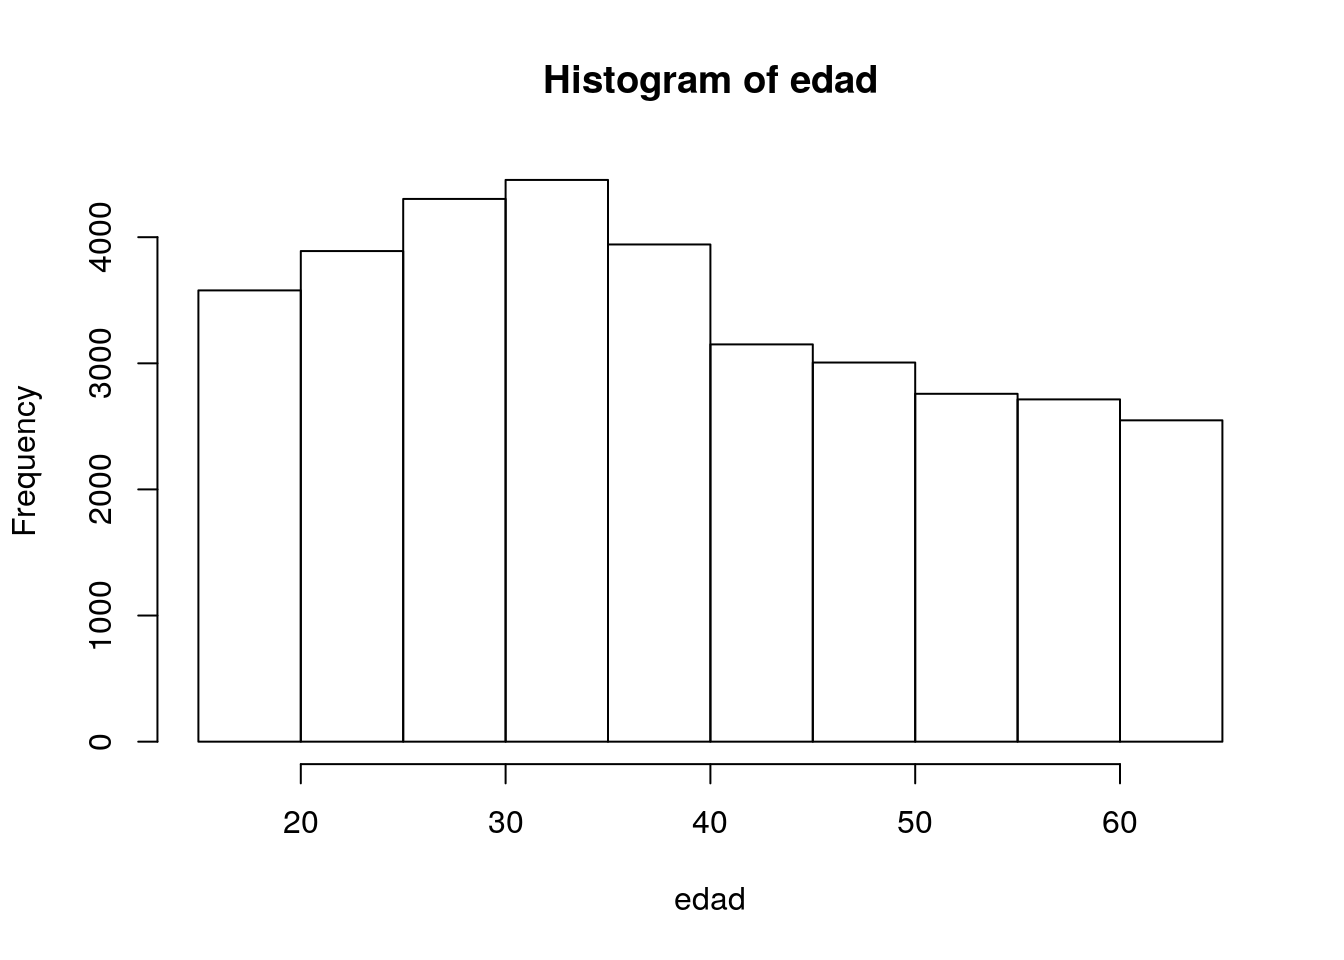
\includegraphics{Introduccion_Datos_files/figure-latex/unnamed-chunk-31-1.pdf}

También podemos representar las frecuencias relativas o los porcentajes.

\begin{Shaded}
\begin{Highlighting}[]
\NormalTok{## Realizamos un histograma con las frecuencias relativas}
\KeywordTok{library}\NormalTok{(lattice)}
\KeywordTok{histogram}\NormalTok{(edad,}
          \DataTypeTok{breaks =} \DecValTok{10}\NormalTok{,}
          \DataTypeTok{ylab =} \StringTok{"Porcentaje del Total"}\NormalTok{)}
\end{Highlighting}
\end{Shaded}

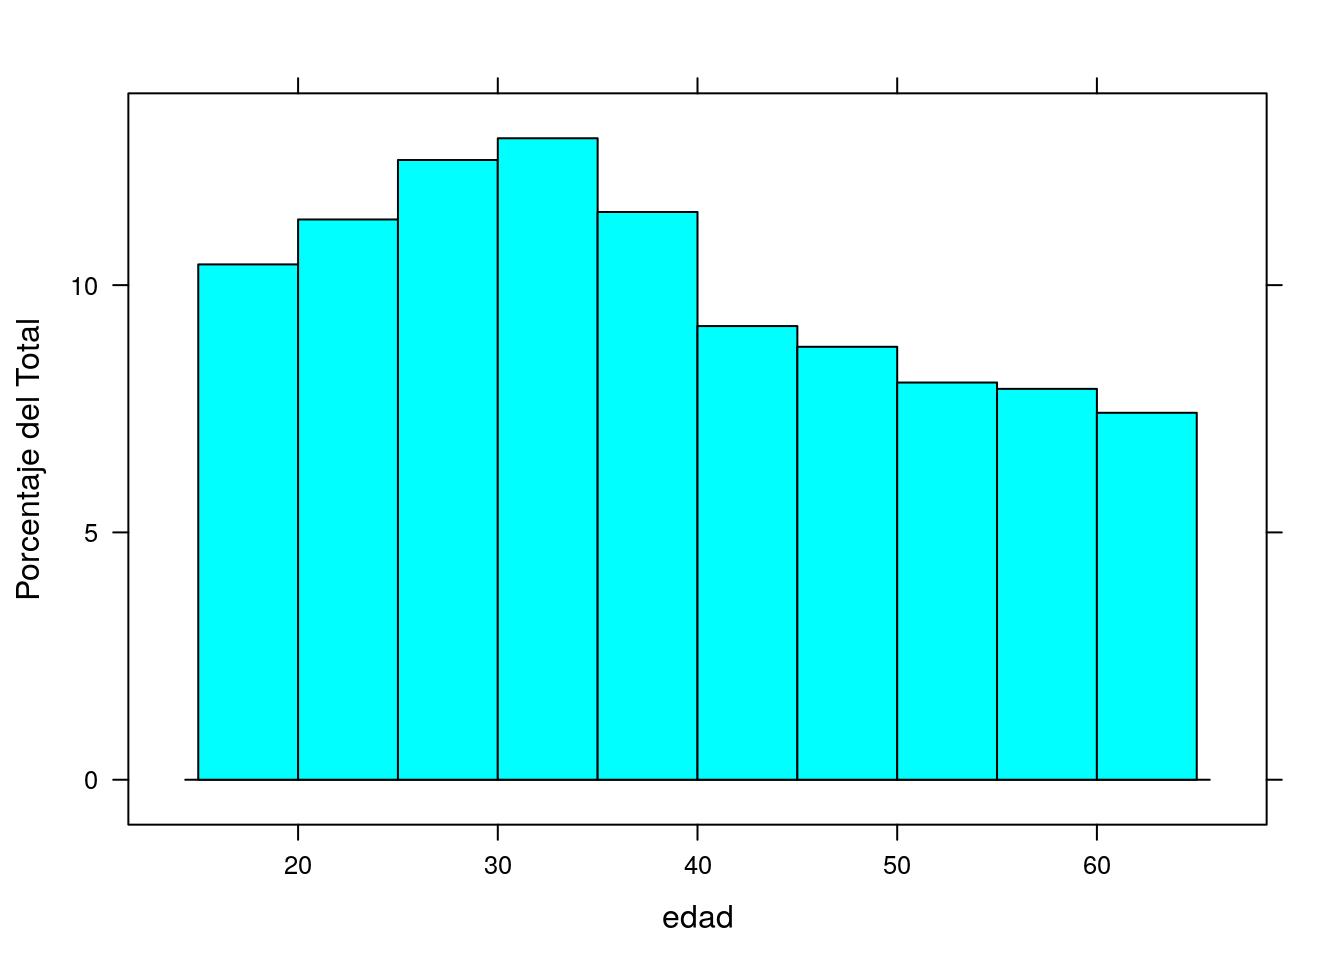
\includegraphics{Introduccion_Datos_files/figure-latex/unnamed-chunk-32-1.pdf}

\begin{Shaded}
\begin{Highlighting}[]
\NormalTok{## Cambiamos el número de barras. Agregamos color}
\KeywordTok{hist}\NormalTok{(}\KeywordTok{as.numeric}\NormalTok{(edad),}
     \DataTypeTok{col =} \StringTok{"seagreen"}\NormalTok{)}
\end{Highlighting}
\end{Shaded}

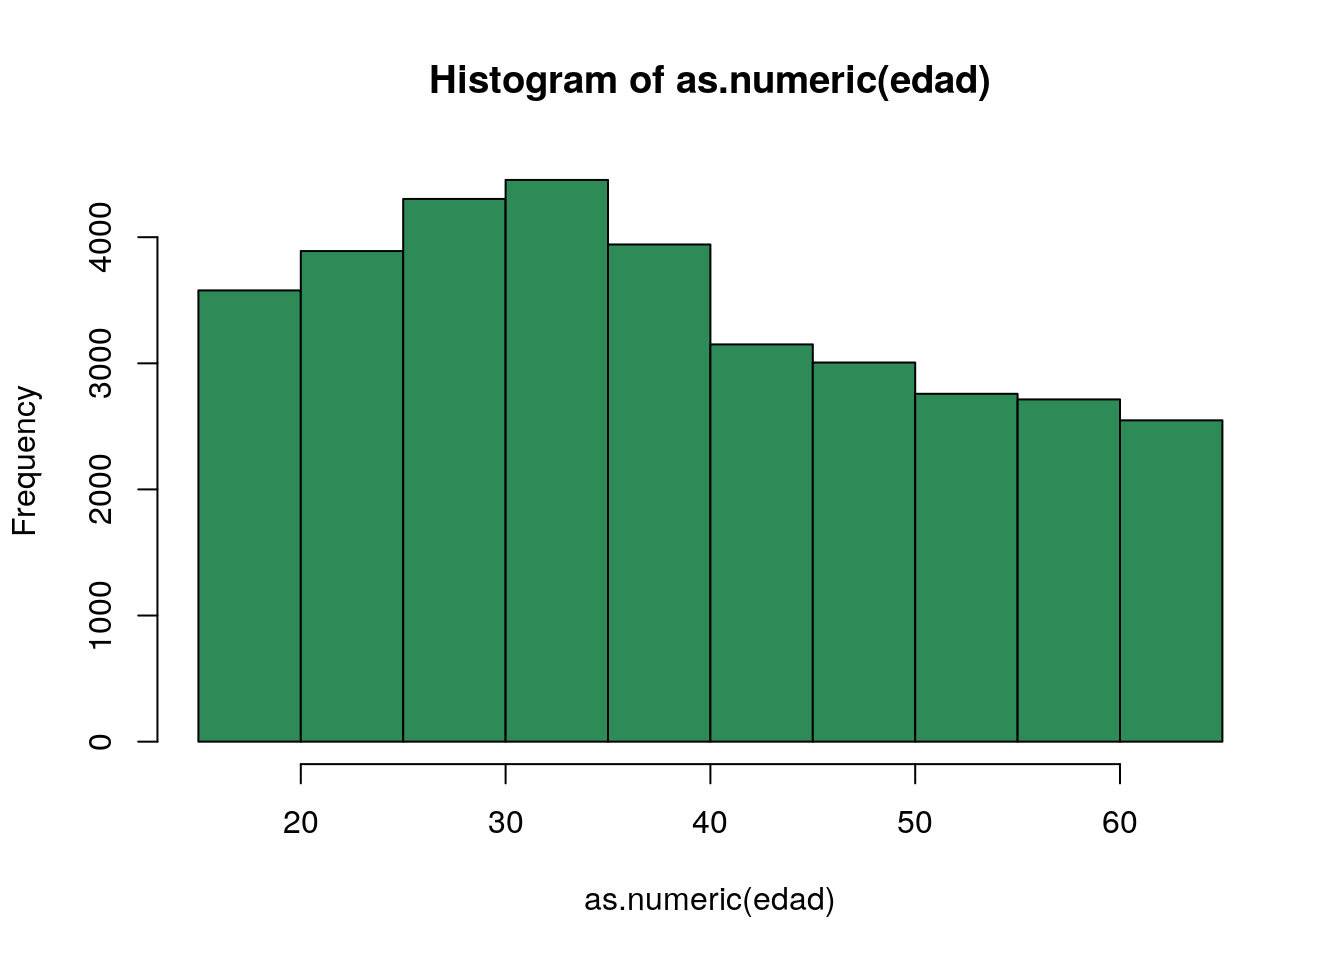
\includegraphics{Introduccion_Datos_files/figure-latex/unnamed-chunk-32-2.pdf}

\begin{Shaded}
\begin{Highlighting}[]
\NormalTok{## Estilamos el gráfico}
\KeywordTok{hist}\NormalTok{(}\KeywordTok{as.numeric}\NormalTok{(edad),}
     \DataTypeTok{axes =} \OtherTok{FALSE}\NormalTok{,}
     \DataTypeTok{main =} \StringTok{"Histograma para edad"}\NormalTok{,}
     \DataTypeTok{xlab =} \StringTok{"Edad"}\NormalTok{,}
     \DataTypeTok{ylab =} \StringTok{"Frecuencia"}\NormalTok{,}
     \CommentTok{# col = "steelblue",}
     \DataTypeTok{xlim =} \KeywordTok{c}\NormalTok{(}\DecValTok{10}\NormalTok{,}\DecValTok{70}\NormalTok{),}
     \DataTypeTok{ylim =} \KeywordTok{c}\NormalTok{(}\DecValTok{0}\NormalTok{, }\DecValTok{5000}\NormalTok{),}
     \DataTypeTok{col =} \KeywordTok{rainbow}\NormalTok{(}\DecValTok{5}\NormalTok{))}
\KeywordTok{axis}\NormalTok{(}\DecValTok{1}\NormalTok{, }\DataTypeTok{pos =} \DecValTok{0}\NormalTok{)}
\KeywordTok{axis}\NormalTok{(}\DecValTok{2}\NormalTok{, }\DataTypeTok{pos =} \DecValTok{10}\NormalTok{)}
\end{Highlighting}
\end{Shaded}

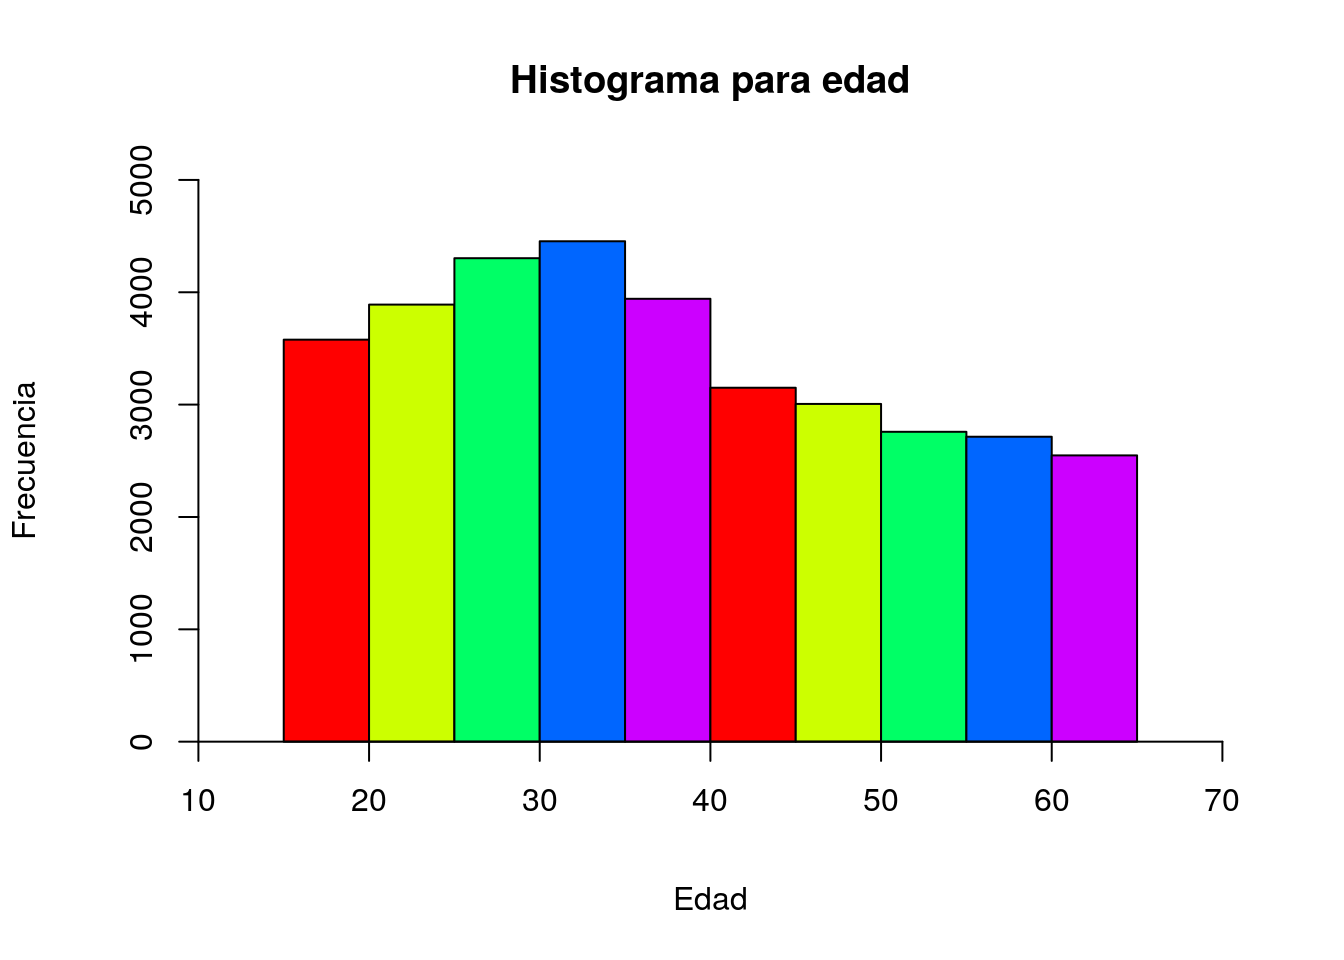
\includegraphics{Introduccion_Datos_files/figure-latex/unnamed-chunk-32-3.pdf}

\section{Gráfico de barras}\label{grafico-de-barras}

El gráfivo de barras nos permite visualizar las frecuencias en
\textbf{variables cualitativas}.

\begin{Shaded}
\begin{Highlighting}[]
\NormalTok{## Seleccionamos BISG02 y la guardamos en una nueva variable}
\NormalTok{accidente <-}\StringTok{ }\NormalTok{enprecosp}\OperatorTok{$}\NormalTok{BISG02}

\NormalTok{## Convertimos a factor y etiquetamos los códigos de valores}
\NormalTok{accidente <-}\StringTok{ }\KeywordTok{factor}\NormalTok{(accidente,}
                    
                   \DataTypeTok{labels =} \KeywordTok{c}\NormalTok{(}\StringTok{"Sí"}\NormalTok{, }\StringTok{"No"}\NormalTok{, }\StringTok{"Ns/Nc"}\NormalTok{))}
\NormalTok{## Construimos las frecuencias para la variable accidente}
\NormalTok{f <-}\StringTok{ }\KeywordTok{table}\NormalTok{(accidente)}
\NormalTok{frel <-}\StringTok{ }\KeywordTok{prop.table}\NormalTok{(f)}

\NormalTok{## Juntamos todo y armamos una tabla de distribución de freucuencias.}
\NormalTok{dfreq <-}\StringTok{ }\KeywordTok{cbind}\NormalTok{(f, frel)}

\KeywordTok{barplot}\NormalTok{(dfreq[,}\DecValTok{1}\NormalTok{],}
        \DataTypeTok{col =} \StringTok{"steelblue"}\NormalTok{)}
\end{Highlighting}
\end{Shaded}

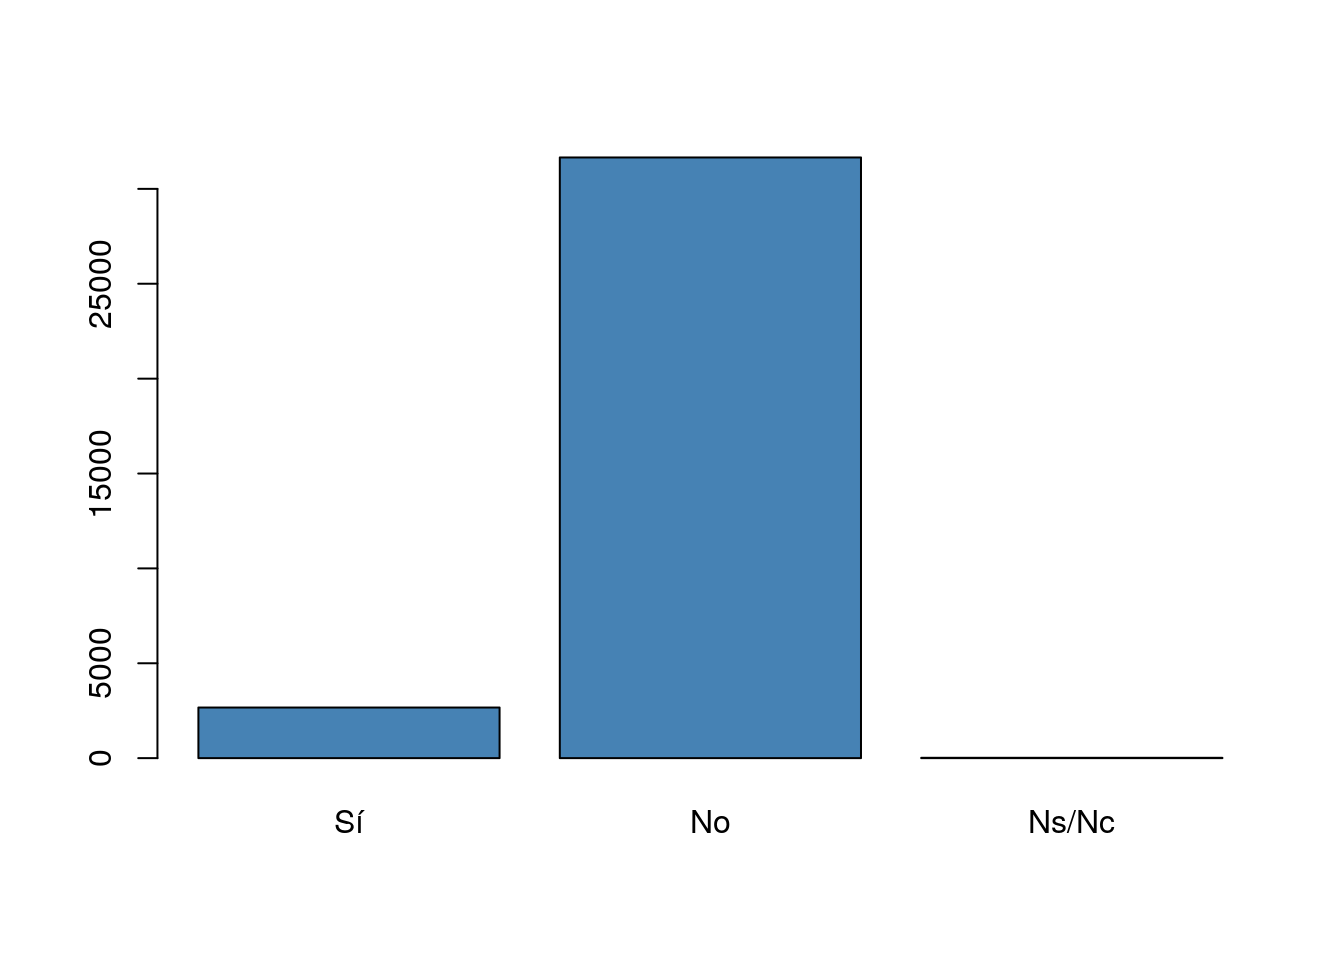
\includegraphics{Introduccion_Datos_files/figure-latex/unnamed-chunk-33-1.pdf}

\section{Gráfico de tortas}\label{grafico-de-tortas}

Los gráficos de tortas también nos permiten graficar frecuencias. Los
gráficos de torta están actualmente desaconsejados. Se aconseja en su
lugar el uso de gráfico de barras. Los gráficos de barras permiten
visualizar más facilemente las diferencias de proporciones que los
gráficos de barras, particularmente cuando representamos más de dos
proporciones. Para ver una revisión acerca de la discusión de gráficos
de barras y de torta vea \citet{spence2005no}.

Entonces

\bibliography{book.bib,packages.bib}


\end{document}
